\section{Mean energy per pair and the Fano factor}\label{sec:18.2}

A \SI{5.9}{keV} X-ray absorbed in silicon at \SI{123}{K} leaves on average 1574 electron--hole pairs. If each pair were an independent event, the count would scatter by $\sqrt{1574} = 39.7$ from one X-ray to the next. The measured spread is 13.7, a Fano factor $F_{\mathrm{eh}} = 0.119$ at a mean energy per pair $\varepsilon_{\mathrm{eh}} = \SI{3.749}{eV}$ (\cref{tab:18-pairs}). These two numbers fix where the bins of one, two and three pairs sit on the axis of deposited energy, and how sharp they are. The cascade of \cref{sec:18.1} produces both. A pair that costs more heat leaves less energy for the pairs that follow, and this constraint, not the randomness of each collision, makes the count sub-Poissonian.

\subsection{Moments of the heat}\label{sec:18.2-heat}

Every event of the cascade obeys the energy identity \cref{eq:18.1-energy}, $\omega = N_{\mathrm{eh}}\Eg + E_{\mathrm{heat}}$, as long as no carrier is captured, no exciton forms and no photon leaves the crystal before the pairs are counted; \cref{sec:18.5} removes each of these conditions. At fixed $\omega$ the pair number and the heat are therefore one random variable, not two. Taking the mean and the variance of the identity at fixed $\omega$, with $\bar n = \langle N_{\mathrm{eh}}\rangle$ the mean pair number,
\begin{equation}
  \varepsilon_{\mathrm{eh}} = \frac{\omega}{\bar n} = \Eg + \frac{\langle E_{\mathrm{heat}}\rangle}{\bar n} , \qquad
  F_{\mathrm{eh}} = \frac{\operatorname{Var}N_{\mathrm{eh}}}{\bar n} = \frac{\operatorname{Var}E_{\mathrm{heat}}}{\Eg^2\,\bar n} .
  \label{eq:18.2-moments}
\end{equation}
Both ratios depend on $\omega$ for small deposits. The symbols $\varepsilon_{\mathrm{eh}}$ and $F_{\mathrm{eh}}$ denote their limits at large $\omega$, where $\bar n$ and $\operatorname{Var}N_{\mathrm{eh}}$ grow in proportion to $\omega$ (\cref{sec:18.2-linear}). $F_{\mathrm{eh}}$ has nothing to do with the Fano coefficients $c^{\mathrm{F}}_\nu$ of \cref{eq:8.6-fano}, which describe the interference of a discrete state with a continuum; the two carry the name of the same physicist.

The cascade makes its heat in two ways. Let $E_<$ be the kinetic energy that each carrier holds when it falls below the threshold $\theta_{\mathrm{ii}}\Eg$ for good, summed over carriers. That carrier then relaxes to its band edge by emitting phonons, but the amount is fixed at the moment it becomes terminal. Let $E_>$ be the energy of the phonons emitted while carriers are still above threshold. With $E_{\mathrm{heat}} = E_< + E_>$, expanding the variance in \cref{eq:18.2-moments} gives
\begin{keyresult}[Fano factor as cascade moments]
\begin{equation}
  F_{\mathrm{eh}} = \mathcal{V}_< + \mathcal{V}_> + 2\mathcal{V}_{<>} , \qquad
  \mathcal{V}_< = \frac{\operatorname{Var}E_<}{\Eg^2\,\bar n} , \quad
  \mathcal{V}_> = \frac{\operatorname{Var}E_>}{\Eg^2\,\bar n} , \quad
  \mathcal{V}_{<>} = \frac{\operatorname{Cov}(E_<, E_>)}{\Eg^2\,\bar n} ,
  \label{eq:18.2-decomp}
\end{equation}
together with $\varepsilon_{\mathrm{eh}} = \omega/\bar n$, in the limit of large $\omega$. Each term is a variance or covariance of an additive deposit of the cascade, computed by the moment recursions of \cref{app:D.43}.
\end{keyresult}
\noindent The decomposition itself is an identity. Its content is that every term can be computed. A deposit is additive if each collision adds a fixed amount to it: one unit of $N_{\mathrm{eh}}$ per ionization, $\omega_{\mathrm{AB}}$ to $E_>$ per phonon emitted above threshold, and $x$ to $E_<$ when a carrier at kinetic energy $x$ becomes terminal. For such a deposit the first and second moments $m_t(x)$ and $M_t(x)$ obey \cref{eq:D.43-m1,eq:D.43-m2}, the energy-only form of the recursions \cref{eq:C.11-mean,eq:C.11-second}. We condition on the first collision of a carrier, and the three products of an ionization start independent subtrees whose moments are already known at lower energy. After a phonon emission the carrier continues at $x - \omega_{\mathrm{AB}}$. The variances in \cref{eq:18.2-decomp} are $M_t - m_t^2$ for the deposits $E_<$ and $E_>$, and the covariance follows from the second moment of $E_< - E_>$, a route independent of the two variances.

The model is the random-$k$ cascade of \cref{sec:18.1-reductions}. Both carriers have free-particle densities of states $\rho_t(x) \propto x^{1/2}$, and the hole density of states stops at the valence band width $B_{\mathrm{h}}$. The threshold ratio is $\theta_{\mathrm{ii}} = 1$, and one optical phonon of energy $\omega_{\mathrm{AB}}$ competes with ionization through the rate ratio \cref{eq:18.1-randomk}. Measured in units of the gap, the cascade then depends on the crystal through two numbers, $\lambda_{\mathrm{AB}} = A_{\mathrm{AB}}/\Eg^3$ and $w_{\mathrm{AB}} = \omega_{\mathrm{AB}}/\Eg$. The first sets the strength of phonon emission relative to impact ionization: one gap above threshold, at $x = 2\Eg$, the rate ratio \cref{eq:18.1-randomk} is $(105/2\pi)(2 - w_{\mathrm{AB}})^{1/2}\lambda_{\mathrm{AB}} = 23.3\,\lambda_{\mathrm{AB}}$. The second is the energy lost in one phonon step. For silicon at \SI{123}{K}, $\Eg = \SI{1.160}{eV}$~\cite[Eq.~(11)]{ramanathan2020ionization}, $\omega_{\mathrm{AB}} = \SI{63}{meV}$ and $B_{\mathrm{h}} = \SI{12}{eV}$ (\cref{app:E.13}). With the one constant that \cref{sec:18.4} fixes by the measured pair energy, $A_{\mathrm{AB}} = \SI{5.703}{eV^3}$, silicon has $\lambda_{\mathrm{AB}} = 3.654$ and $w_{\mathrm{AB}} = 0.0543$. The seed is an electron with all of $\omega - \Eg$, its hole at the band edge. The slopes of $\bar n$ and $\operatorname{Var}N_{\mathrm{eh}}$ in $\omega$, fitted for seed energies between $20\Eg$ and $40\Eg$, give $\varepsilon_{\mathrm{eh}} = 3.232\,\Eg = \SI{3.749}{eV}$ and $F_{\mathrm{eh}} = 0.114$. In practice the recursions are solved on grids of step $\Eg/74$ and $\Eg/148$ and extrapolated to zero step (\cref{app:D.43}). A first-principles cascade would replace both kernels by those of \cref{sec:18.1}; \cref{app:E.24} sets it up so that the three terms of \cref{eq:18.2-decomp} come out separately.

For a single deposit the slopes are only the end point. The approach to them is set by the constant terms of the mean and the variance, $\bar n = \omega/\varepsilon_{\mathrm{eh}} + b_N + o(1)$ and $\operatorname{Var}N_{\mathrm{eh}} = F_{\mathrm{eh}}\omega/\varepsilon_{\mathrm{eh}} + c_N + o(1)$, whose existence \cref{sec:18.2-linear} discusses. The constant $b_N$ depends on the seed (\cref{sec:18.3-limits}), and for the one-sided seed of silicon $c_N = -0.02$. The pair energy at finite $\omega$ lies below its limit by the fraction $b_N\varepsilon_{\mathrm{eh}}/\omega$.

\begin{limitbox}[Pair energy and Fano factor of a finite deposit][lim:18.2a]
The energy-dependent pair energy and Fano factor $\varepsilon(\omega) = \omega/\bar n(\omega)$ and $F(\omega) = \operatorname{Var}N_{\mathrm{eh}}(\omega)/\bar n(\omega)$ tend to constants at high energy~\cite[Eqs.~(2)--(3)]{ramanathan2020ionization}; the constants are the cascade moments $\varepsilon_{\mathrm{eh}}$ and $F_{\mathrm{eh}}$ of \cref{eq:18.2-decomp}.
\par\smallskip
{\centering
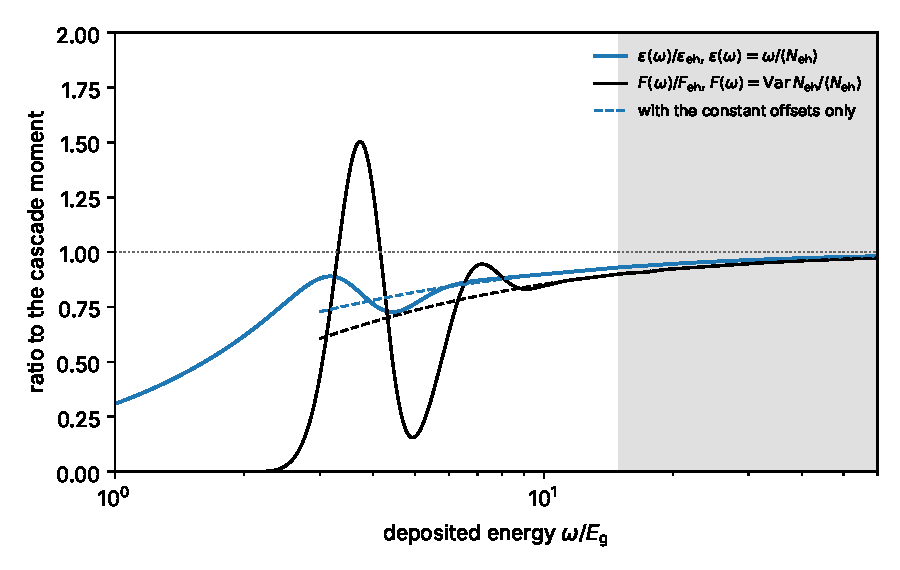
\includegraphics[width=\linewidth]{figures/ch18/limit18_2a.pdf}
\captionof{figure}{Pair energy (blue) and Fano factor (black) of a deposit $\omega$ in silicon, in units of their high-energy limits $\varepsilon_{\mathrm{eh}} = 3.232\,\Eg$ and $F_{\mathrm{eh}} = 0.114$, against $\omega/\Eg$. Energy-only random-$k$ cascade with $\Eg = \SI{1.160}{eV}$, $\omega_{\mathrm{AB}} = \SI{63}{meV}$, $A_{\mathrm{AB}} = \SI{5.703}{eV^3}$, $\theta_{\mathrm{ii}} = 1$, hole band width \SI{12}{eV}; seed electron with all of $\omega - \Eg$, hole at the band edge; moment recursions on a grid of step $\Eg/74$, the ratios taken on that grid. Dashed: the limits corrected by the constant terms only, $\varepsilon(\omega)/\varepsilon_{\mathrm{eh}} = (1 + b_N\varepsilon_{\mathrm{eh}}/\omega)^{-1}$ and $F(\omega)/F_{\mathrm{eh}} = (1 + c_N\varepsilon_{\mathrm{eh}}/F_{\mathrm{eh}}\omega)(1 + b_N\varepsilon_{\mathrm{eh}}/\omega)^{-1}$, with the constant terms of this seed fitted between 30 and $60\Eg$ ($b_N$ of \cref{sec:18.3-limits}, $c_N = -0.02$; the slopes are fitted between 20 and $40\Eg$). Gray: $\omega \ge 14.9\,\Eg = \SI{17.3}{eV}$, where both ratios lie within \SI{10}{\percent} of 1.}\label{fig:18-limit-moments}
\par}
\smallskip
Below about $15\Eg$ the yield rises in steps of one pair, and $F(\omega)$ swings between 0 and $1.5\,F_{\mathrm{eh}}$, so that a search at a few pairs needs the full distribution of the pair number (\cref{sec:18.3}) rather than two moments.
\end{limitbox}

At $\omega \le 2\Eg$ the seed electron cannot ionize and $F(\omega) = 0$: one pair, always. The first ionizations then make the variance rise and fall as each new pair becomes possible. Above $10\Eg$ the constant terms describe the approach to within \SI{1}{\percent}: at $\omega = 10\Eg$ the computed ratios differ from the dashed curves by \SI{0.07}{\percent} in $\varepsilon$ and \SI{0.9}{\percent} in $F$.

\subsection{The three variance terms in silicon}\label{sec:18.2-silicon}

In silicon the three terms of \cref{eq:18.2-decomp} are $\mathcal{V}_< = 0.092$, $\mathcal{V}_> = 0.290$ and $2\mathcal{V}_{<>} = -0.268$, and they add to $F_{\mathrm{eh}} = 0.114$. The largest term is not the residual energy below threshold but the phonon energy above it. The mean phonon energy emitted above threshold is \SI{0.92}{eV} per pair, about 15 phonons of \SI{63}{meV}. If those phonons were independent emissions, their number would be Poisson, $\operatorname{Var}E_> = \omega_{\mathrm{AB}}\langle E_>\rangle$, and $\mathcal{V}_> = w_{\mathrm{AB}}\langle E_>\rangle/(\Eg\bar n) = 0.043$. The computed term is 6.7 times larger. The reason is the steep energy dependence of \cref{eq:18.1-randomk}. Within a few phonon steps of threshold the probability that the next collision ionizes is below $10^{-4}$; it is 0.004 at \SI{2}{eV} and reaches a few percent only at 2.5 to \SI{3}{eV} (\cref{app:E.13}). As a result, a carrier in this range emits a run of phonons whose length has a long, nearly geometric tail. Two carriers that start at the same energy can end their runs many phonons apart.

Most of this variance is canceled by the covariance, which removes \SI{92}{\percent} of $\mathcal{V}_>$. Energy conservation along each carrier line ties the two heats together. A carrier that emits more phonons just above threshold either falls below threshold with a smaller residual, or ionizes later, at a lower energy, into smaller products. What a long run of phonons adds to $E_>$, it takes from $E_<$. The net Fano factor is therefore a small difference of two large terms, which has a practical consequence for any calculation: an error of \SI{1}{\percent} in $\mathcal{V}_>$ alone moves $F_{\mathrm{eh}}$ by \SI{2.5}{\percent}. The covariance is the correlation between the two kinds of heat along one line of descent, not between sibling carriers.

\Cref{fig:18-decomp} follows the three terms as phonon emission grows stronger, at the phonon step of silicon. Without phonons, $E_> = 0$ and $F_{\mathrm{eh}} = \mathcal{V}_<$ is pure partition noise: the scatter of the residual energies with which the carriers end, 0.081 for parabolic bands at $\theta_{\mathrm{ii}} = 1$. At $\lambda_{\mathrm{AB}} = 0.003$ the phonon term is still small, $\mathcal{V}_> = 0.009$, and the covariance is positive, $+0.010$. From $\lambda_{\mathrm{AB}} \approx 0.1$ on, both large terms grow, until at $\lambda_{\mathrm{AB}} = 30$ they reach $\mathcal{V}_> = 0.55$ and $2\mathcal{V}_{<>} = -0.61$. Across these four decades $F_{\mathrm{eh}}$ itself rises only from 0.085 to 0.132, and for $\lambda_{\mathrm{AB}}$ between 1 and 10 it stays between 0.105 and 0.122. In this model a Fano factor near 0.11 is generic for a semiconductor. A full-band cascade of silicon with no fitted constant gives the same 0.114 (\cref{sec:18.4-three}). The measured value tests the shape of the rate ratio within a few phonon energies of threshold, where the two large terms are made, more than it tests the constant $A_{\mathrm{AB}}$ (\cref{sec:18.4}).

\begin{figure}[tbp]
  \centering
  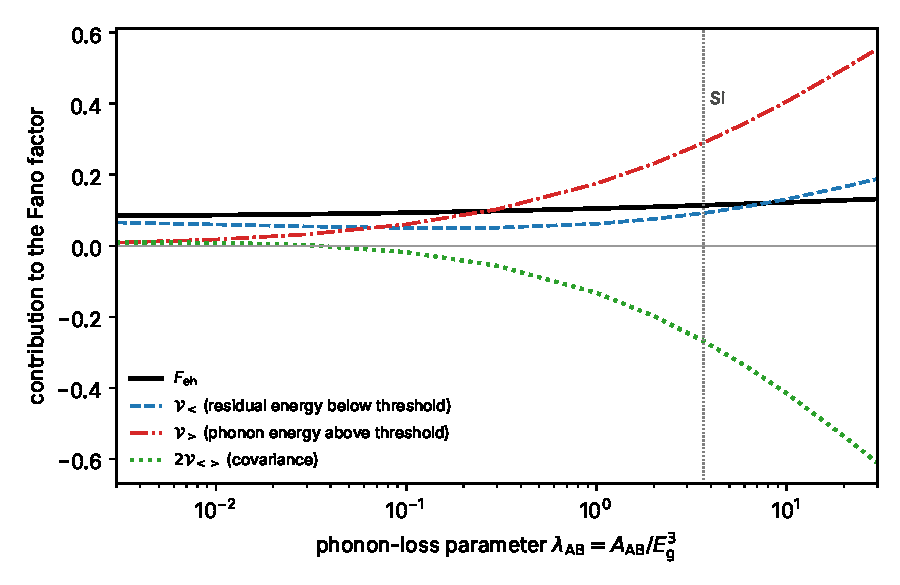
\includegraphics[width=0.85\linewidth]{figures/ch18/fig18_2.pdf}
  \caption{Fano factor $F_{\mathrm{eh}}$ (solid) and its three terms, \cref{eq:18.2-decomp}, against the phonon-loss parameter $\lambda_{\mathrm{AB}} = A_{\mathrm{AB}}/\Eg^3$ at the phonon step of silicon, $w_{\mathrm{AB}} = \omega_{\mathrm{AB}}/\Eg = 0.0543$. Dashed: $\mathcal{V}_<$, from the residual energies of the carriers when they fall below threshold; dash-dotted: $\mathcal{V}_>$, from the phonon energy emitted above threshold; dotted: $2\mathcal{V}_{<>}$, their covariance. Energy-only random-$k$ cascade with parabolic densities of states, $\theta_{\mathrm{ii}} = 1$, hole band width $12\,\mathrm{eV}/\Eg$; asymptotic slopes for seed energies between $X/2$ and $X$, $X = 40\Eg$ ($60\Eg$ for $\lambda_{\mathrm{AB}} > 5$); moment recursions on grids of step $\Eg/74$ and $\Eg/148$, extrapolated to zero step. The vertical line marks silicon, $\lambda_{\mathrm{AB}} = 3.654$, where the terms are $0.092 + 0.290 - 0.268 = 0.114$.}
  \label{fig:18-decomp}
\end{figure}

\subsection{The random-parking limit}\label{sec:18.2-parking}

One limit of the cascade has an exact solution. Take a constant electron density of states, a valence band so narrow that every hole is born at the band edge, $\theta_{\mathrm{ii}} = 1$, and no phonons. An electron of kinetic energy $x \ge \Eg$ then ionizes into a hole at rest and two electrons that share $x - \Eg$ with uniform probability, since the joint density of states of \cref{eq:18.1-phase} is flat on the line $x_1 + x_2 = x - \Eg$. In units of $\Eg$ this is the random parking problem of R\'enyi~\cite{subashiev2010correlation}. A car of unit length parks at a uniformly random place in a free gap of length $x$ and leaves two gaps, which are filled in the same way until every gap is shorter than a car. The jamming density $\rho_\infty$, the number of cars per unit length at the end, is the number of pairs per unit energy, so that $\varepsilon_{\mathrm{eh}} = \Eg/\rho_\infty$. Subashiev and Luryi proposed this limit as a test of Fano-factor models, since both moments are known exactly~\cite[Sect.~I]{subashiev2010correlation}. \Cref{we:18-parking} derives them from the recursions of \cref{sec:18.2-heat}.

\begin{workedexample}{The random-parking Fano factor}\label{we:18-parking}
Measure energies in units of $\Eg$. Let $M(x)$ be the mean number of new pairs made by an electron of kinetic energy $x$. The hole of each ionization is terminal with zero residual, and the two electrons share $x - 1$ uniformly, so \cref{eq:C.11-mean} with one pair per ionization reads $M(x) = 0$ for $x < 1$ and
\begin{equation*}
  M(x) = 1 + \frac{2}{x - 1}\int_0^{x - 1}M(y)\,\dd y , \qquad x \ge 1 .
\end{equation*}
Put $x = z + 1$ and multiply by $z$: $zM(z + 1) = z + 2\int_0^zM(y)\,\dd y$. Take the Laplace transform $m(s) = \int_0^\infty\ee^{-sx}M(x)\,\dd x$. Since $M$ vanishes below 1, the transform of $M(z + 1)$ is $\ee^sm(s)$, and multiplication by $z$ becomes $-\dd/\dd s$. With $\phi(s) = \ee^sm(s)$,
\begin{equation*}
  \phi'(s) + \frac{2\ee^{-s}}{s}\,\phi(s) = -\frac{1}{s^2} , \qquad
  \phi(s) = \int_s^\infty\frac{\dd t}{t^2}\,\exp\bigl[2E_1(s) - 2E_1(t)\bigr] ,
\end{equation*}
the solution that vanishes as $s \to \infty$, with $E_1(s) = \int_s^\infty\ee^{-u}u^{-1}\dd u$ the exponential integral. For every $s > 0$, exactly, $E_1(s) = -\gamma_{\mathrm{E}} - \ln s + \mathrm{Ein}(s)$, with Euler's constant $\gamma_{\mathrm{E}}$ and $\mathrm{Ein}(s) = \int_0^s(1 - \ee^{-u})u^{-1}\dd u \to 0$. Hence $\ee^{2E_1(s)} \to \ee^{-2\gamma_{\mathrm{E}}}/s^2$ as $s \to 0$, and inserting the same identity for $E_1(t)$ under the integral,
\begin{equation*}
  m(s) \to \frac{\rho_\infty}{s^2} , \qquad
  \rho_\infty = \int_0^\infty\exp\bigl[-2\,\mathrm{Ein}(t)\bigr]\,\dd t = 0.74759792 .
\end{equation*}
A double pole $\rho_\infty/s^2$ is the transform of $\rho_\infty x$, so $M(x) \to \rho_\infty x$: the pair energy is $\varepsilon_{\mathrm{eh}} = \Eg/\rho_\infty = 1.3376\,\Eg$. The second moment obeys \cref{eq:C.11-second} with the same kernel. Solved on grids of step 0.01 and 0.005 and extrapolated linearly in the step, it yields $F_{\mathrm{eh}} = 0.051040$ and $1/\varepsilon_{\mathrm{eh}} = 0.747599$, against the closed form $F_{\mathrm{park}} = 0.0510387$~\cite[Eq.~(44)]{subashiev2010correlation}.

The renewal estimate of \cref{sec:18.2-renewal} needs only the final state. At jamming, the number of gaps of size $g$ per unit length is~\cite[Eq.~(19)]{subashiev2010correlation}
\begin{equation*}
  G(g) = 2\int_0^\infty t\,\exp\bigl[-gt - 2\,\mathrm{Ein}(t)\bigr]\,\dd t , \qquad 0 \le g \le 1 .
\end{equation*}
Each gap is the residual energy of one terminal electron, and there is one per pair. Integrating, $\int G\,\dd g = \rho_\infty$ (one gap per car) and $\int(1 + g)G\,\dd g = 1$ (cars and gaps fill the line), both to 30 digits. Each pair costs $1 + g$, with $\langle g\rangle = 0.337617 = 1/\rho_\infty - 1$ and $\operatorname{Var}g = 0.079437$, so that \cref{eq:18.2-ren} gives
\begin{equation*}
  F_{\mathrm{ren}} = \frac{\operatorname{Var}g}{(1 + \langle g\rangle)^2} = 0.0443977 = 0.870\,F_{\mathrm{park}} .
\end{equation*}
The final-state statistics are exact here, and still the estimate misses \SI{13}{\percent} of the Fano factor. (The values printed in Ref.~\cite{subashiev2010correlation}, $\rho_\infty = 0.7475987$ and 0.0439766, carry misprints in the seventh and third digits.)
\end{workedexample}

Silicon is far from this limit in two ways. Its densities of states rise as $x^{1/2}$, and phonons compete with ionization. The density of states alone, at $\lambda_{\mathrm{AB}} \to 0$, raises $\varepsilon_{\mathrm{eh}}$ from $1.338\,\Eg$ to $1.585\,\Eg$ and $F_{\mathrm{eh}}$ from 0.051 to 0.081. \Cref{lim:18.2b} keeps the parking kernel and adds the phonons.

\begin{limitbox}[Random-parking limit][lim:18.2b]
For a constant electron density of states, holes born at the band edge, $\theta_{\mathrm{ii}} = 1$ and no phonons, the cascade is R\'enyi's random parking, with $\Eg/\varepsilon_{\mathrm{eh}} = \rho_\infty = \int_0^\infty\ee^{-2\,\mathrm{Ein}(t)}\dd t = 0.74759792$~\cite[Eq.~(23)]{subashiev2010correlation} and $F_{\mathrm{eh}} = F_{\mathrm{park}} = 0.0510387$~\cite[Eq.~(44)]{subashiev2010correlation}.
\par\smallskip
{\centering
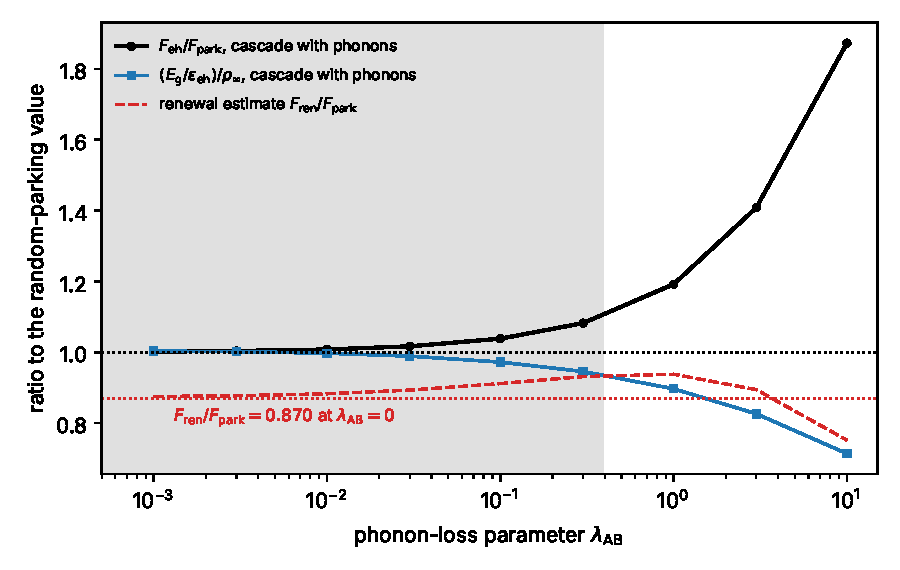
\includegraphics[width=\linewidth]{figures/ch18/limit18_2b.pdf}
\captionof{figure}{The parking kernel with phonons: $F_{\mathrm{eh}}/F_{\mathrm{park}}$ (black) and $(\Eg/\varepsilon_{\mathrm{eh}})/\rho_\infty$ (blue) against $\lambda_{\mathrm{AB}}$, with one phonon step $w_{\mathrm{AB}} = 0.0543$ (silicon) and the phonon-to-ionization ratio $\lambda_{\mathrm{AB}}/(x/\Eg - 1)$ of \cref{eq:18.1-randomk} for a constant density of states, where $\mathfrak{P}(y) = y$ and $A_{\mathrm{AB}}$ carries eV, so that here $\lambda_{\mathrm{AB}} = A_{\mathrm{AB}}/\Eg$. Dashed red: the renewal estimate $F_{\mathrm{ren}}$ of \cref{eq:18.2-rencasc}; dotted red: its parking value 0.870. Moment recursions on a grid of step $\Eg/74$, which places the values at $\lambda_{\mathrm{AB}} \to 0$ \SI{0.4}{\percent} ($\rho$) and \SI{0.1}{\percent} ($F$) above the exact ones. Gray: $\lambda_{\mathrm{AB}} < 0.40$, where both ratios are within \SI{10}{\percent} of 1 (bisection in $\ln\lambda_{\mathrm{AB}}$).}\label{fig:18-limit-park}
\par}
\smallskip
For $\lambda_{\mathrm{AB}} \gtrsim 0.4$ the carriers lose their last energy above threshold to phonons, which lowers the pair density and raises $F_{\mathrm{eh}}$, the trend that carries the parking values toward those of silicon.
\end{limitbox}

Relative to the parking values computed on the same grid, the phonons lower $\Eg/\varepsilon_{\mathrm{eh}}$ and raise $F_{\mathrm{eh}}$ by $0.8\,\lambda_{\mathrm{AB}}$ for $\lambda_{\mathrm{AB}} \le 0.003$, and by \SI{3.2}{\percent} and \SI{3.7}{\percent} at $\lambda_{\mathrm{AB}} = 0.1$. At $\lambda_{\mathrm{AB}} = 3$ the parking kernel leads to $F_{\mathrm{eh}} = 0.072$, 1.41 times $F_{\mathrm{park}}$; the rest of the way to the 0.114 of silicon is the shape of the densities of states.

\subsection{The renewal estimate}\label{sec:18.2-renewal}

A shortcut to $F_{\mathrm{eh}}$ uses only the statistics of the final state. Suppose that each pair costs the gap plus a heat $c_i$, that the costs are independent and identically distributed with mean $\varepsilon_{\mathrm{eh}} - \Eg$ and variance $\sigma_{\mathrm{pair}}^2$, and that pairs are made until $\omega$ is spent. This is the single renewal chain of \cref{app:C.11} with one loss per pair, and \cref{eq:C.11-fano} gives $\operatorname{Var}N_{\mathrm{eh}} \simeq \sigma_{\mathrm{pair}}^2\omega/\varepsilon_{\mathrm{eh}}^3$, that is,
\begin{equation}
  F_{\mathrm{ren}} = \frac{\sigma_{\mathrm{pair}}^2}{\varepsilon_{\mathrm{eh}}^2} ,
  \label{eq:18.2-ren}
\end{equation}
the uncorrelated final-state estimate of Subashiev and Luryi~\cite[Eq.~(7)]{subashiev2010correlation}. The denominator is $\varepsilon_{\mathrm{eh}}$, not $\Eg$. With $N_{\mathrm{eh}}$ held fixed, the heat would scatter by $\bar n\sigma_{\mathrm{pair}}^2$, and \cref{eq:18.2-moments} would give $\sigma_{\mathrm{pair}}^2/\Eg^2$. At fixed $\omega$, however, a pair that costs more heat leaves less energy for the pairs after it, and this constraint multiplies the variance by $(\Eg/\varepsilon_{\mathrm{eh}})^2$.

In a cascade the costs are built from computed statistics. Each pair ends with one terminal electron and one terminal hole, whose residual energies have the variances $\sigma_{\mathrm{e}}^2$ and $\sigma_{\mathrm{h}}^2$, and the phonon heat above threshold is taken as Poisson. Then
\begin{equation}
  F_{\mathrm{ren}} = \frac{\sigma_{\mathrm{e}}^2 + \sigma_{\mathrm{h}}^2 + \omega_{\mathrm{AB}}\langle E_>\rangle/\bar n}{\varepsilon_{\mathrm{eh}}^2} ,
  \label{eq:18.2-rencasc}
\end{equation}
which keeps the one-carrier statistics of the final state exactly and drops every correlation. In random parking it is the gap-law value 0.0443977 of \cref{we:18-parking}. \Cref{lim:18.2c} compares it with the full $F_{\mathrm{eh}}$.

\begin{limitbox}[Renewal estimate of the Fano factor][lim:18.2c]
For independent, identically distributed costs per pair with variance $\sigma_{\mathrm{pair}}^2$, the Fano factor is $F_{\mathrm{ren}} = \sigma_{\mathrm{pair}}^2/\varepsilon_{\mathrm{eh}}^2$~\cite[Eq.~(7)]{subashiev2010correlation}, built for the cascade as \cref{eq:18.2-rencasc}.
\par\smallskip
{\centering
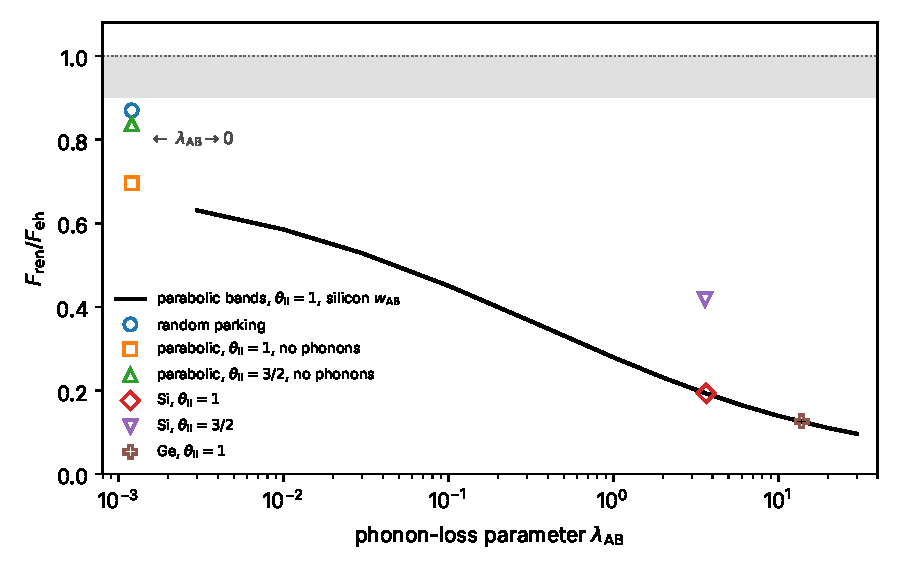
\includegraphics[width=\linewidth]{figures/ch18/limit18_2c.pdf}
\captionof{figure}{Ratio of the renewal estimate \cref{eq:18.2-rencasc} to the full Fano factor \cref{eq:18.2-decomp} against $\lambda_{\mathrm{AB}}$. Line: parabolic densities of states, $\theta_{\mathrm{ii}} = 1$, $w_{\mathrm{AB}} = 0.0543$, hole band width $12\,\mathrm{eV}/\Eg$ (the kernel of \cref{fig:18-decomp}). Markers at $\lambda_{\mathrm{AB}} \to 0$, extrapolated from grid steps 0.01 and $0.005\,\Eg$: random parking (0.870), parabolic bands without phonons at $\theta_{\mathrm{ii}} = 1$ (0.696) and $3/2$ (0.837). Further markers: silicon at $\theta_{\mathrm{ii}} = 1$ (0.193) and at $\theta_{\mathrm{ii}} = 3/2$ with $A_{\mathrm{AB}}$ recalibrated to the pair energy, \SI{5.629}{eV^3} (0.418); germanium with $\Eg = \SI{0.744}{eV}$, $\omega_{\mathrm{AB}} = \SI{37.6}{meV}$, the silicon $A_{\mathrm{AB}}$ and the hole density of states cut at the germanium valence-band width, \SI{12.6}{eV}~\cite[Table~II]{rideau2006strained} (0.126). Markers and line are continuum limits of the moment recursions. The gray band, within \SI{10}{\percent} of the full value, contains no computed case.}\label{fig:18-limit-renewal}
\par}
\smallskip
The estimate drops the correlations of the cascade, all of which raise the variance here: it lies below $F_{\mathrm{eh}}$ in every computed case, by \SI{13}{\percent} in random parking, by a factor 5 in silicon and by a factor 8 in germanium.
\end{limitbox}

The ratio falls from 0.70 to 0.10 as $\lambda_{\mathrm{AB}}$ grows, because the phonon heat above threshold is far from Poisson (\cref{sec:18.2-silicon}), while \cref{eq:18.2-rencasc} counts it as Poisson and has no covariance term at all. Without phonons the gap is smaller but still there: $F_{\mathrm{eh}} - F_{\mathrm{ren}} = 0.025$ at $\theta_{\mathrm{ii}} = 1$ and 0.013 at $\theta_{\mathrm{ii}} = 3/2$, with exact one-carrier statistics. This difference measures every departure from independent, identical costs together: correlations between the products of one ionization, between the electron and the hole of one pair, and between distant carriers, and the differences between the cost laws of different pairs. It does not isolate any one of them. In random parking Subashiev and Luryi find the correlation correction positive at intermediate filling and at jamming, and they note that correlations between the two halves of a split are not the only ones~\cite[Sect.~IV]{subashiev2010correlation}. A Fano factor fitted with a final-state model therefore needs a broader residual distribution, or a larger phonon variance, than the cascade actually has.

\subsection{The linear mean yield}\label{sec:18.2-linear}

The definitions \cref{eq:18.2-moments} assume that $\bar n$ grows in proportion to $\omega$. For a single chain of independent losses, \cref{app:C.11} proved this with the key renewal theorem, \cref{eq:C.11-linear}. The cascade is not a single chain, since an ionization splits the energy among three carriers, and no loss law is common to all its steps. The leading term still follows from renewal theory if we follow a unit of energy instead of a carrier. Give each ionization of a carrier at kinetic energy $x$ the weight 1, spread evenly over the $x$ units of energy that the carrier holds. The number of ionizations in a cascade started at kinetic energy $E$ is then the integral of the collected weights over all units. Taking the mean,
\begin{equation}
  \bar n_{\mathrm{sub}}(E) = E\,\Bigl\langle\sum_j\frac{1}{x_j}\Bigr\rangle_u ,
  \label{eq:18.2-tagged}
\end{equation}
where $u$ is a unit chosen uniformly in $[0, E]$, the sum runs over the ionizations along the chain of carriers that hold $u$, $x_j$ is the kinetic energy of the holder at the $j$-th of them, and $\langle\cdots\rangle_u$ is the mean over $u$ and over the cascade. A holder that emits phonons first ionizes below the energy at which it received the unit; $x_1 = E$ only if the first collision of the seed carrier is an ionization. The carriers that hold one unit form a chain. At an ionization the unit passes to one of the three products with probability equal to that product's share of the energy, or it leaves the chain into the gap of the new pair, with probability $\Eg/x$. At a phonon emission it leaves with probability $\omega_{\mathrm{AB}}/x$. \Cref{app:D.44} shows that \cref{eq:18.2-tagged} is exact for any branching law that conserves energy.

At high energy the shares no longer depend on $x$. In the random-$k$ model the products divide $x - \Eg$ in proportions whose law tends to a fixed law, and the probability of leaving into the gap falls as $\Eg/x$. The logarithm $\ln x_j$ thus performs a random walk with steps $\ln(x_{j+1}/x_j) \le 0$ whose law becomes independent of $x$. By the renewal theorem in the variable $\ln x$, the distribution with which the walk first arrives in the region within a few gaps of threshold converges as $E \to \infty$. The sum in \cref{eq:18.2-tagged} is dominated by that region, since the high-energy terms are small, $1/x_j$ each. Its mean converges. With the seed pair counted,
\begin{keyresult}[Linear mean yield]
\begin{equation}
  \bar n(\omega) = \frac{\omega}{\varepsilon_{\mathrm{eh}}} + o(\omega) , \qquad
  \frac{1}{\varepsilon_{\mathrm{eh}}} = \lim_{E\to\infty}\Bigl\langle\sum_j\frac{1}{x_j}\Bigr\rangle_u ,
  \label{eq:18.2-linear}
\end{equation}
for any energy-conserving cascade whose share law becomes independent of the energy at high energy, approaches that limit fast enough, is not concentrated on a lattice in $\ln x$, and is regular near threshold. \Cref{app:D.44} states the four conditions and gives the proof.
\end{keyresult}
\noindent The share law must be spread out in $\ln x$. A cascade that always splits in fixed proportions would make the walk lattice, and $\bar n/\omega$ would oscillate in $\ln\omega$ forever instead of converging.

Two statements that the definitions also use are not part of \cref{eq:18.2-linear}. The first is the constant term $b_N$, which depends on the seed (\cref{sec:18.3-limits}). In the one-phonon model every energy loss is a whole combination of $\Eg$ and $\omega_{\mathrm{AB}}$, and as for the deterministic chain of \cref{app:C.11} the constant then carries a periodic remainder that never dies out. We can therefore fit the slopes over a range of seed energies, $[X/2, X]$, which averages the remainder. The second is the linear growth of the variance, $\operatorname{Var}N_{\mathrm{eh}} = F_{\mathrm{eh}}\omega/\varepsilon_{\mathrm{eh}} + O(1)$, which the computed slopes obey but which needs the same second-order estimates as $b_N$.

\subsection{Constant term and the renewal bound}\label{sec:18.2-open}

The constant term and the variance of the yield at second order in renewal theory have not been derived for the branching cascade. The expansions $\bar n = \omega/\varepsilon_{\mathrm{eh}} + b_N + o(1)$ and $\operatorname{Var}N_{\mathrm{eh}} = F_{\mathrm{eh}}\omega/\varepsilon_{\mathrm{eh}} + O(1)$ need second-order estimates for the walk of \cref{eq:18.2-tagged} and the rate at which the cascade forgets its seed, and neither is in hand. The constant matters at a few pairs: at \SI{10}{eV} in silicon, $\omega/\varepsilon_{\mathrm{eh}} = 2.67$, and the constant term of the one-sided seed adds \SI{13}{\percent} to it. The second open question is whether the renewal estimate \cref{eq:18.2-rencasc} is a lower bound on $F_{\mathrm{eh}}$ for every cascade of this class. It is in every case computed here and in random parking, but there is no proof. A proof would make the final-state statistics a guaranteed floor for the Fano factor, and a counterexample would show which correlations can lower the variance.
